\documentclass[10pt,twocolumn,a4paper]{article}

%% ── Geometry ──────────────────────────────────────────────────────────────────
\usepackage[top=1in,bottom=1in,left=0.75in,right=0.75in,columnsep=0.25in]{geometry}

%% ── Core packages ─────────────────────────────────────────────────────────────
\usepackage{cite}
\usepackage{hyperref}
\usepackage{amsmath,amssymb}
\usepackage{array,booktabs,tabularx,boldline,multirow,makecell}
\usepackage{setspace,parskip}
\usepackage{titlesec}
\usepackage{xcolor}
\usepackage{abstract}
\usepackage{graphicx}
\usepackage{enumitem}
\usepackage{adjustbox}
\usepackage{caption}

%% ── TikZ ──────────────────────────────────────────────────────────────────────
\usepackage{tikz}
\usetikzlibrary{arrows.meta,positioning,shapes,fit,backgrounds,calc}

%% ── Hyperref colours ─────────────────────────────────────────────────────────
\hypersetup{colorlinks=true,linkcolor=black,citecolor=blue,urlcolor=blue}

%% ── Section formatting ────────────────────────────────────────────────────────
\titleformat{\section}{\normalfont\normalsize\bfseries\scshape}{\Roman{section}.}{0.5em}{}
\titleformat{\subsection}{\normalfont\normalsize\itshape}{\Alph{subsection}.}{0.5em}{}
\titlespacing*{\section}{0pt}{6pt}{3pt}
\titlespacing*{\subsection}{0pt}{4pt}{2pt}

%% ── Abstract formatting ───────────────────────────────────────────────────────
\renewcommand{\abstractnamefont}{\normalfont\bfseries}
\renewcommand{\abstracttextfont}{\normalfont\small}
\setlength{\absleftindent}{0pt}
\setlength{\absrightindent}{0pt}
\setlength{\textfloatsep}{8pt plus 2pt minus 2pt}
\setlength{\floatsep}{6pt plus 2pt minus 2pt}
\setlength{\intextsep}{7pt plus 2pt minus 2pt}
\setlength{\dbltextfloatsep}{8pt plus 2pt minus 2pt}
\setlength{\dblfloatsep}{7pt plus 2pt minus 2pt}
\captionsetup{font=small,labelfont=bf,skip=4pt}

%% ── Custom colours ────────────────────────────────────────────────────────────
\definecolor{novelty}{RGB}{0,100,60}    % dark green for implemented labels
\definecolor{proposed}{RGB}{100,60,0}   % amber for proposed labels

%% ── Title ─────────────────────────────────────────────────────────────────────
\title{\large\textbf{Privacy-Preserving Blockchain Framework for Organ Donation:%
 ZKP-Authenticated Role-Scoped Functional Encryption with%
 GDPR-Compliant IPFS Storage}}

\author{
  \normalsize Chirag Parmar\\
  \small M250738CS\\[2pt]
  \normalsize Guided by: Dr.~Abidha V.P \& Dr.~Bijoy Das\\
  \small Department of Computer Science and Engineering, NIT Calicut
}

\date{September 2026}

%% ══════════════════════════════════════════════════════════════════════════════
\begin{document}
\maketitle
\thispagestyle{empty}

%% ── Abstract ──────────────────────────────────────────────────────────────────
\begin{abstract}
\noindent
Organ donation and transplantation systems face critical challenges in participant
authentication, data confidentiality, and regulatory compliance. Existing
blockchain-based solutions expose sensitive donor--recipient attributes in plaintext,
rely on pseudonymous Ethereum addresses that violate GDPR pseudonymisation
requirements, and lack standardised data lifecycle management. This Phase~II report
extends the Phase~I literature survey with a detailed proposed architecture and a
working prototype implementation. The proposed system integrates three novel components
that no single prior work combines: (i)~Zero-Knowledge Proof~(ZKP) role
authentication based on a Poseidon Merkle-inclusion circuit~(5,\!391 constraints,
Groth16/BN128), which gates the issuance of role-scoped Polynomial Functional
Encryption~(PFE) keys; (ii)~antigen-level ABO/Rh compatible homomorphic
scoring~(5~BFV ciphertexts per record, Microsoft~SEAL); and (iii)~GDPR
Article~17-compliant data lifecycle management via smart-contract-triggered IPFS
unpinning. The prototype, implemented with Hardhat/Solidity~0.8.20, circom~2.2.3,
snarkjs, and a React~18 frontend, achieves~62/62 unit tests and~69+ integration tests
passing. Real measured benchmarks confirm the system's feasibility: Groth16
on-chain proof verification consumes~375,\!645 gas, BFV encryption runs in~20.9\,ms,
and polynomial evaluation completes in~26.6\,ms.

\smallskip\noindent
\textbf{Keywords:} Blockchain; IPFS; Polynomial Functional Encryption; Zero-Knowledge
Proofs; Organ Transplantation; Homomorphic Encryption; GDPR; Privacy-Preserving
Authentication; Role-Based Access Control; Post-Quantum Cryptography.
\end{abstract}

%% ══════════════════════════════════════════════════════════════════════════════
\section{Introduction}
%% ══════════════════════════════════════════════════════════════════════════════

Organ transplantation is one of the most logistically and ethically demanding
workflows in modern healthcare. Every step---donor registration, medical screening,
donor--recipient matching, organ allocation, transport, and post-transplant record
management---demands simultaneous guarantees of data integrity, participant
authenticity, privacy, and regulatory compliance. Globally, approximately twenty
patients die daily while awaiting a matched donor~\cite{hawashin2022}. Centralised
organ registries are susceptible to data breaches, unauthorised access, fraudulent
matching, and organ trafficking.

Blockchain technology provides a tamper-proof, auditable, and decentralised
record-keeping substrate~\cite{hawashin2022,mewada2026}. Prior work has demonstrated
Ethereum-based organ lifecycle management~\cite{hawashin2022}, encrypted compatibility
scoring via Polynomial Functional Encryption (PFE)~\cite{samsukha2025}, and
Personal Health Record~(PHR) protection using Fully Homomorphic Encryption~(FHE) with
IPFS off-chain storage~\cite{vanin2023}. However, blockchain transparency is also
a liability: all on-chain activity is permanently linked to Ethereum addresses,
violating GDPR pseudonymisation requirements~(Art.~4(5)) when an address can be
correlated with a real-world identity.

Zero-Knowledge Proofs~(ZKPs)~\cite{goldwasser1989,ranaweera2023} address this gap by
allowing a participant to prove role membership without revealing their credential or
identity. When combined with PFE key issuance---where the smart contract issues a
functional secret key~$sk_f$ only upon successful ZKP verification---access control
becomes cryptographically enforced at the function level, not merely at the identity
level. This integration, first proposed in our Phase~I survey, has been identified as
absent from all reviewed literature, including the most closely related prior work,
Block-Privacy~\cite{egala2023}, which combines ZKP, functional encryption, and IPFS
for IoMT but does not address organ-specific polynomial scoring or role-scoped key
issuance.

This Phase~II report makes the following contributions:
\begin{enumerate}[leftmargin=*, nosep]
  \item A detailed system architecture describing the ZKP authentication pipeline,
        PFE key issuance, IPFS-backed ciphertext storage, and GDPR lifecycle
        management~(\S\ref{sec:arch}).
  \item A working prototype implementation with real Groth16 on-chain proofs,
        antigen-level ABO/Rh homomorphic compatibility scoring, and an automated
        GDPR revocation path~(\S\ref{sec:impl}).
  \item Empirical performance benchmarks including gas costs, proof times, and
        SEAL~BFV timings~(\S\ref{sec:impl}).
  \item A brief security analysis demonstrating ZKP soundness, GDPR compliance,
        and replay attack prevention~(\S\ref{sec:security}).
\end{enumerate}

%% ══════════════════════════════════════════════════════════════════════════════
\section{Literature Review}
\label{sec:litreview}
%% ══════════════════════════════════════════════════════════════════════════════

\subsection{Blockchain-Based Organ Donation Management}

Hawashin et al.~\cite{hawashin2022} proposed the most complete organ lifecycle system
to date: a private Ethereum blockchain encoding donor registration, waiting-list
management, auto-matching, organ removal, delivery, and transplantation in two Solidity
smart contracts. Six stakeholder roles are each assigned a unique Ethereum address with
role-restricted function calls. The system was validated using the Oyente tool with
EVM code coverage of 80.9\% and 99.1\%, confirming the absence of re-entrancy,
integer overflow, and MITM vulnerabilities. However, all medical attributes---blood
type, BMI, age, organ type---are stored and processed in \emph{plaintext}; no
off-chain storage, encryption, or ZKP authentication is employed. Mewada et
al.~\cite{mewada2026} reviewed blockchain solutions for organ transplant transparency,
confirming the systematic absence of cryptographic privacy mechanisms across reviewed
implementations. The Blockchain-Enabled Organ Matching System~(BOMS)~\cite{boms2024}
incorporates biological matching into smart contract logic but relies on Ethereum
addresses for identity---a weak pseudonymisation mechanism vulnerable to
de-anonymisation through address clustering or off-chain correlation.

\subsection{Functional and Homomorphic Encryption for Medical Privacy}

Samsukha et al.~\cite{samsukha2025} presented the most directly relevant prior work:
a PFE framework for encrypted organ compatibility scoring combining
Composable-Functional-Encryption security~(CFE-security)~\cite{matt2015}, the BFV
Homomorphic Encryption~(HE) scheme, and the Hungarian algorithm on the Ethereum
Sepolia testnet. The compatibility polynomial
\begin{equation}
  f(\mathbf{x}) = \beta_0 + \beta_1 x_1 + \beta_2 x_2 + \beta_3 x_3
                + \beta_4 x_1 x_2 + \beta_5 x_2 x_3
  \label{eq:pfe-samsukha}
\end{equation}
encodes blood type~($x_1$), HLA aggregate score~($x_2$), and urgency~($x_3$) as a
single-bit blood-type variable and an aggregate HLA score, benchmarking 464
donor--recipient pairs in under one second. Key limitations: no IPFS implementation
(referenced only as future work), no ZKP participant authentication, no post-transplant
data lifecycle management, and a clinically incomplete polynomial (no antigen-level
ABO/Rh decomposition, no ischemia time, no DSA status).

Cheon et al.~\cite{cheon2020} established the theoretical foundation for PFE with a
linear ciphertext size~$O(\ell)$ independent of polynomial degree~$d$, which Samsukha
et al.~\cite{samsukha2025} adopt. Matt and Maurer~\cite{matt2015} formalised
CFE-security within the constructive cryptography framework.

Vanin et al.~\cite{vanin2023} proposed a PHR protection model combining blockchain,
IPFS, and FHE~(BFV via Microsoft SEAL). The Data Steward~(DS) and Shared Data
Vault~(SDV) roles implement time-bounded IPFS storage with JWT-based consent windows;
post-expiry, DS nodes unpin IPFS files. Evaluated on 1.285~million COVID-19 records,
FHE computation completes in under three minutes, but 100,\!000 records require
$\approx$7\,GB of storage and block propagation of 10,\!000 encrypted records across
100~nodes takes hours. The authors explicitly acknowledge the absence of a complete
data retirement module. Hegde et al.~\cite{hegde2025} confirmed that HE-based
encrypted clinical computation achieves near-baseline accuracy~(98.6\% vs.\
98.7\% baseline for CKD classification) but at a $20\times$ ciphertext expansion and
26\% training-round overhead under CKKS.

\subsection{Zero-Knowledge Proof Authentication in Healthcare Blockchains}

Bai et al.~\cite{bai2022} proposed Health-zkIDM, a ZKP-based identity system for
healthcare built on Hyperledger Fabric. ZKP authentication prevents on-chain
transactions from being linked to real-world patient identities, directly addressing
GDPR pseudonymisation. Luong and Park~\cite{luong2022} demonstrated that zk-SNARK
proofs can be verified by Ethereum smart contracts for privacy-preserving identity
management, confirming practical gas cost bounds for on-chain ZKP verification.
Bharath~Babu and Jothi~\cite{bharathbabu2024} showed that zk-SNARK-based analytics
authentication in multi-tenant cloud EHR environments can operate within acceptable
gas limits. Diro et al.~\cite{diro2024} surveyed 47~ZKP-blockchain identity schemes
and identified the critical open challenge: \emph{no existing scheme integrates ZKP
identity verification with functional encryption-based fine-grained data access
control}---precisely the gap the proposed system addresses. Ranaweera et
al.~\cite{ranaweera2023} demonstrated ZKP for EHR access control on blockchain,
confirming the applicability of Poseidon-based circuits to healthcare identity. Zhou
et al.~\cite{zhou2024} designed a ZKP-based donation scheme with auditability
(EISDSPA), confirming that ZKP and blockchain auditability are compatible in
donation contexts.

\subsection{IPFS-Integrated Off-Chain Storage}

Jayabalan and Jeyanthi~\cite{jayabalan2022} established the canonical IPFS-on-chain
architecture for healthcare: encrypted patient records stored on IPFS, content
identifiers~(CIDs) registered on-chain, with time-bounded smart-contract-enforced
access revocation. The study confirms that the CID-on-chain pattern consistently
outperforms full on-chain storage in throughput, latency, and cost. The
GDPR-compliant Personal Health Record sharing mechanism of~\cite{gdprtdsc2023}
combined redactable blockchain with IPFS unpinning to approximate the Right to
Erasure~(GDPR Art.~17), providing the design template for the LifecycleManager
contract in the proposed system.

\subsection{Most Closely Related Prior Work: Block-Privacy}

Egala et al.~\cite{egala2023} proposed Block-Privacy, a privacy-preserving smart
healthcare framework for Internet-of-Medical-Things~(IoMT) that integrates
blockchain, IPFS, ZKP, and functional encryption. This is the closest single prior
work to the proposed system. However, four key differences distinguish the proposed
system: (i)~Block-Privacy targets general IoMT data access control with
general~FE, whereas the proposed system uses PFE polynomial evaluation for
organ-specific compatibility scoring; (ii)~Block-Privacy's ZKP authenticates device
identity generically, whereas the proposed system implements six organ-donation-specific
role circuits with permission bitmasks enforced in the PFE key issuance step;
(iii)~the proposed system implements antigen-level ABO/Rh homomorphic
compatibility---a clinically meaningful improvement absent from Block-Privacy;
(iv)~the proposed system demonstrates a complete GDPR Art.~17 revocation path via
LifecycleManager~$\to$~RevocationExecuted~$\to$~IPFS~unpin, which Block-Privacy
does not address. Both papers share the high-level design philosophy; the proposed
system instantiates it for the organ donation domain with clinically grounded and
formally benchmarked implementation.

%% ══════════════════════════════════════════════════════════════════════════════
\section{Research Gaps}
\label{sec:gaps}
%% ══════════════════════════════════════════════════════════════════════════════

Table~\ref{tab:litreview} compares the five most relevant prior works across the
architectural axes of the proposed system.

\begin{table*}[!t]
\centering
\caption{Comparative analysis: existing works vs.\ proposed system.}
\label{tab:litreview}
\renewcommand{\arraystretch}{1.18}
\scriptsize
\setlength{\tabcolsep}{5pt}
\begin{tabularx}{\textwidth}{>{\raggedright\arraybackslash}p{2.05cm} *{5}{>{\centering\arraybackslash}X}}
\toprule
\textbf{Criterion}
  & \textbf{Hawashin \cite{hawashin2022}}
  & \textbf{Samsukha \cite{samsukha2025}}
  & \textbf{Vanin \cite{vanin2023}}
  & \textbf{Block-Privacy \cite{egala2023}}
  & \textbf{Proposed} \\
\midrule
Domain & Organ life-cycle & Organ matching & PHR sharing & IoMT & Organ donation \\
Blockchain & Private Ethereum & Ethereum Sepolia & Permissioned & Permissioned & Permissioned Ethereum \\
IPFS off-chain & \textcolor{red}{None} & Ref.\ only & \checkmark & \checkmark & \checkmark \\
Encryption & \textcolor{red}{None} & PFE+HE & FHE/BFV & General FE & PFE/BFV \\
ZKP authentication & \textcolor{red}{No} & \textcolor{red}{No} & \textcolor{red}{No} & \checkmark\ (general) & \checkmark\ (role) \\
ZKP gates FE key & \textcolor{red}{No} & \textcolor{red}{No} & \textcolor{red}{No} & \textcolor{red}{No} & \textcolor{green!60!black}{\checkmark} \\
ABO/Rh accuracy & \textcolor{red}{Plaintext} & 1-bit & N/A & N/A & \textcolor{green!60!black}{Antigen-level} \\
Data expiry & \textcolor{red}{No} & \textcolor{red}{No} & Partial & \textcolor{red}{No} & \textcolor{green!60!black}{\checkmark} \\
GDPR Art.~17 & \textcolor{red}{No} & \textcolor{red}{No} & Partial & \textcolor{red}{No} & \textcolor{green!60!black}{\checkmark} \\
PQ-resistant & \textcolor{red}{No} & \textcolor{red}{No} & \textcolor{red}{No} & \textcolor{red}{No} & Planned \\
\bottomrule
\end{tabularx}
\end{table*}

Five principal gaps motivate the proposed design:

\textbf{Gap~1.}\enspace\textit{No ZKP role proof gating PFE key issuance.}
No prior work uses a ZKP as the on-chain authorisation trigger for issuing a
role-scoped PFE functional secret key~$sk_f$. This specific chain---ZKP proof~$\to$
smart-contract 4-check verification~$\to$ role-scoped~$sk_f$ issuance~$\to$ IPFS
ciphertext decryption---is the primary novel contribution.

\textbf{Gap~2.}\enspace\textit{Clinically incomplete compatibility polynomials.}
Samsukha et al.~\cite{samsukha2025} collapse blood type to a single binary
variable~($x_1\in\{0,1\}$), making A+, B+, AB+, and O+ indistinguishable to the
scoring formula. Real ABO/Rh incompatibility requires antigen-level computation:
$\mathrm{incomp} = (\mathrm{donHasA}\wedge\neg\mathrm{recHasA}) +
(\mathrm{donHasB}\wedge\neg\mathrm{recHasB}) + (\mathrm{donHasRh}\wedge\neg\mathrm{recHasRh})$,
evaluated homomorphically over five ciphertexts~$(c_{A}, c_{B}, c_{\mathrm{Rh}},
c_{\mathrm{HLA}}, c_{\mathrm{urg}})$.

\textbf{Gap~3.}\enspace\textit{Absent GDPR/HIPAA-compliant data lifecycle.}
No organ donation system provides automatic, blockchain-logged, post-transplant
IPFS unpinning tied to smart-contract lifecycle events. This violates GDPR
Art.~17~(Right to Erasure) and HIPAA data retention guidelines.

\textbf{Gap~4.}\enspace\textit{No end-to-end IPFS-PFE organ pipeline.}
Samsukha et al.~\cite{samsukha2025} reference IPFS as future work; Block-Privacy
integrates IPFS for general IoMT, not organ-specific BFV ciphertexts. No prior work
delivers a complete round-trip: encrypt organ attributes with BFV~$\to$ upload to
IPFS~$\to$ register CID on-chain~$\to$ retrieve and score homomorphically~$\to$
revoke on LifecycleManager event.

\textbf{Gap~5.}\enspace\textit{Absence of quantum-resistant primitives in organ systems.}
All reviewed organ donation systems use Ethereum's ECDSA, which is
vulnerable to Shor's algorithm. NIST PQC standards~(FIPS~203/204)~\cite{nist2024fips203,nist2024fips204}
have been finalised; organ registries, which retain records for decades, are
high-value targets for harvest-now-decrypt-later attacks. The proposed system
identifies CRYSTALS-Dilithium signature replacement as the primary future
engineering task.

%% ══════════════════════════════════════════════════════════════════════════════
\section{Proposed System Architecture}
\label{sec:arch}
%% ══════════════════════════════════════════════════════════════════════════════

\subsection{Design Goals and Threat Model}

The system is designed for a permissioned Ethereum network~(Proof-of-Authority) shared
among transplant centres, national registries, and regulators. Primary goals:
(i)~end-to-end confidentiality of donor--recipient attributes under BFV;
(ii)~GDPR pseudonymisation via ZKP-based role authentication;
(iii)~GDPR Art.~17 post-transplant record revocation via IPFS unpin;
(iv)~role-scoped data access enforced at the PFE key level;
(v)~tamper-proof audit trail via on-chain events.

The threat model assumes honest-but-curious infrastructure providers, potential
insider adversaries at hospitals, and external attackers attempting identity
de-anonymisation through on-chain correlation. Quantum adversaries are addressed
as future work.

\subsection{ZKP Role Authentication Pipeline}

Participants authenticate by proving, using a Groth16 zk-SNARK, that they know a
credential~$c$ satisfying:
\begin{align}
  \mathit{nullifier} &= \mathrm{Poseidon}(c,\; r) \label{eq:nullifier}\\
  \mathit{commitment} &= \mathrm{Poseidon}(c,\; \mathit{roleId}) \label{eq:commit}\\
  \mathrm{MerkleRoot}(c,\; \mathbf{path}) &= \mathit{root} \label{eq:merkle}
\end{align}
where $r$ is a fresh per-session salt, $\mathbf{path}$ is the 20-level Poseidon
Merkle inclusion path, and $\mathit{root}$ is the role-specific root stored in
\texttt{RoleRegistry}. Equations~\eqref{eq:nullifier}--\eqref{eq:merkle} constitute
the circuit's constraint system~(5,\!391 constraints; Groth16/BN128). Public
inputs~$[\mathit{root}, \mathit{roleId}, \mathit{nullifier}, \mathit{commitment}]$
are submitted with the proof to \texttt{PFEKeyIssuer.verifyAndIssueKey()}, which
performs four on-chain checks:
\begin{enumerate}[leftmargin=*, nosep]
  \item \textbf{Role consistency}: $\mathit{pubInputs}[1] = \mathit{roleId}$.
  \item \textbf{Root match}: $\mathit{pubInputs}[0] = \texttt{RoleRegistry.getRoot}(\mathit{roleId})$.
  \item \textbf{Nullifier replay}: $\mathit{nullifier} \notin \texttt{usedNullifiers}$.
  \item \textbf{BN128 pairing}: \texttt{ZKPVerifier.verifyProof}$(π_A,π_B,π_C,\mathbf{pub})=\top$.
\end{enumerate}
All four checks must pass; any failure reverts the transaction with no state change.

\subsection{PFE-Gated Key Issuance}

Upon successful verification, the contract computes
\begin{equation}
  \mathit{keyCommitment} = \mathtt{keccak256}(
    \mathit{addr} \concat \mathit{roleId} \concat t_{\mathrm{now}} \concat \mathit{perm})
\end{equation}
and registers it with a four-hour TTL. Each role carries a permission bitmask
(Table~\ref{tab:roles}) stored in \texttt{RoleRegistry}. The off-chain PFE
service derives a role-scoped AES-256-GCM key via
$\mathit{roleKey} = \mathrm{HKDF\text{-}SHA256}(\mathit{master},\;
\mathit{roleId}\,\|\,\mathit{keyCommitment})$,
which is the only key that can decrypt BFV-evaluated compatibility scores for that
role.

\begin{table}[!t]
\centering
\caption{Six roles and their permission bitmasks.}
\label{tab:roles}
\renewcommand{\arraystretch}{1.15}
\scriptsize
\setlength{\tabcolsep}{3pt}
\begin{tabularx}{\columnwidth}{l c *{6}{>{\centering\arraybackslash}X}}
\toprule
\textbf{Role} & \textbf{Id} &
\textbf{b0} & \textbf{b1} & \textbf{b2} & \textbf{b3} & \textbf{b4} & \textbf{b5} \\
\midrule
Doctor        & 0 & \checkmark & \checkmark & \checkmark & & & \\
Coordinator   & 1 & \checkmark & \checkmark & \checkmark & \checkmark & & \\
Procurement   & 2 & & & \checkmark & \checkmark & & \\
Matching      & 3 & \checkmark & & \checkmark & & & \\
Transporter   & 4 & & & \checkmark & & \checkmark & \\
Surgeon       & 5 & \checkmark & & \checkmark & & \checkmark & \checkmark \\
\midrule
\multicolumn{8}{>{\raggedright\arraybackslash}p{\columnwidth}}{\scriptsize
b0=viewScore;\ b1=registerDonor;\ b2=viewRecord;\ b3=procure;\ b4=confirmTx;\ b5=triggerRevoke} \\
\bottomrule
\end{tabularx}
\end{table}

\subsection{IPFS-Backed BFV Ciphertext Storage}

Donor and recipient medical attributes are encrypted using the BFV scheme
(Microsoft~SEAL: \texttt{poly\_mod\_degree}$=4096$, \texttt{plain\_mod}$=786433$)
into five ciphertexts per record: $(c_A, c_B, c_{\mathrm{Rh}}, c_{\mathrm{HLA}},
c_{\mathrm{urg}})$. The ciphertext bundle is uploaded to IPFS via the Kubo daemon;
the returned CID string is registered on-chain via
\texttt{OrganRegistry.registerDonor(cidString, bloodType, hlaRoot)}.
No plaintext attribute ever appears on-chain or on IPFS.

\subsection{Homomorphic ABO/Rh Compatibility Scoring}

The compatibility distance between donor~$D$ and recipient~$R$ is evaluated
homomorphically as:
\begin{align}
  d &= W_{\mathrm{blood}} \cdot I + W_{\mathrm{HLA}} \cdot (c_{\mathrm{HLA}}^D
      \ominus c_{\mathrm{HLA}}^R)^{\otimes 2} \notag\\
    &\quad + W_{\mathrm{urg}} \cdot (c_{\mathrm{urg}}^D \ominus c_{\mathrm{urg}}^R
      )^{\otimes 2}
  \label{eq:dist}
\end{align}
where $\ominus$ and $\otimes$ denote homomorphic subtraction and multiplication,
$I = (c_A^D \otimes \overline{c_A^R}) \oplus (c_B^D \otimes \overline{c_B^R})
\oplus (c_{\mathrm{Rh}}^D \otimes \overline{c_{\mathrm{Rh}}^R})$ is the
antigen-level ABO/Rh incompatibility~(three independent single-depth multiplications),
and weights are $W_{\mathrm{blood}}=100$, $W_{\mathrm{HLA}}=200$,
$W_{\mathrm{urg}}=100$ by default. The compatibility score is displayed as
$\mathrm{score} = 1000 - d$ (clamped to $[0,1000]$).

\subsection{GDPR Lifecycle Management}

Post-transplant, a role with bit~5~(\texttt{triggerRevoke}) calls
\texttt{LifecycleManager.requestRevocation(donorId)}, then
\texttt{executeRevocation(donorId, cidString)}, emitting
\texttt{RevocationExecuted(donorId, cid, timestamp)}. The \texttt{ipfsService}
listens for this event via an ethers.js event listener and automatically calls
\texttt{ipfs.pin.rm(cid)}, removing the encrypted record from IPFS. The CID
and event remain on-chain as the legally required audit trail; only the data content
is deleted, satisfying GDPR Art.~17 within the IPFS content-addressing constraint.

\subsection{Smart Contract Architecture}

The system deploys six Solidity~0.8.20 contracts in dependency order:
\texttt{Groth16Verifier}~$\to$ \texttt{ZKPVerifier}~$\to$ \texttt{RoleRegistry}~$\to$
\texttt{PFEKeyIssuer}~$\to$ \texttt{OrganRegistry}~$\to$ \texttt{LifecycleManager}.
\texttt{ZKPVerifier} uses composition over inheritance to wrap
\texttt{Groth16Verifier}, preserving the IZKPVerifier interface while allowing
mock injection for unit testing. \texttt{OrganRegistry} enforces the
\texttt{onlyValidKey} modifier~(checking \texttt{PFEKeyIssuer.isKeyValid(msg.sender)})
and \texttt{hasPermission(msg.sender, bit)} before any state-changing operation.

%% ── Architecture figure (double-column) ───────────────────────────────────────
\begin{figure*}[!t]
\centering
\resizebox{\textwidth}{!}{%
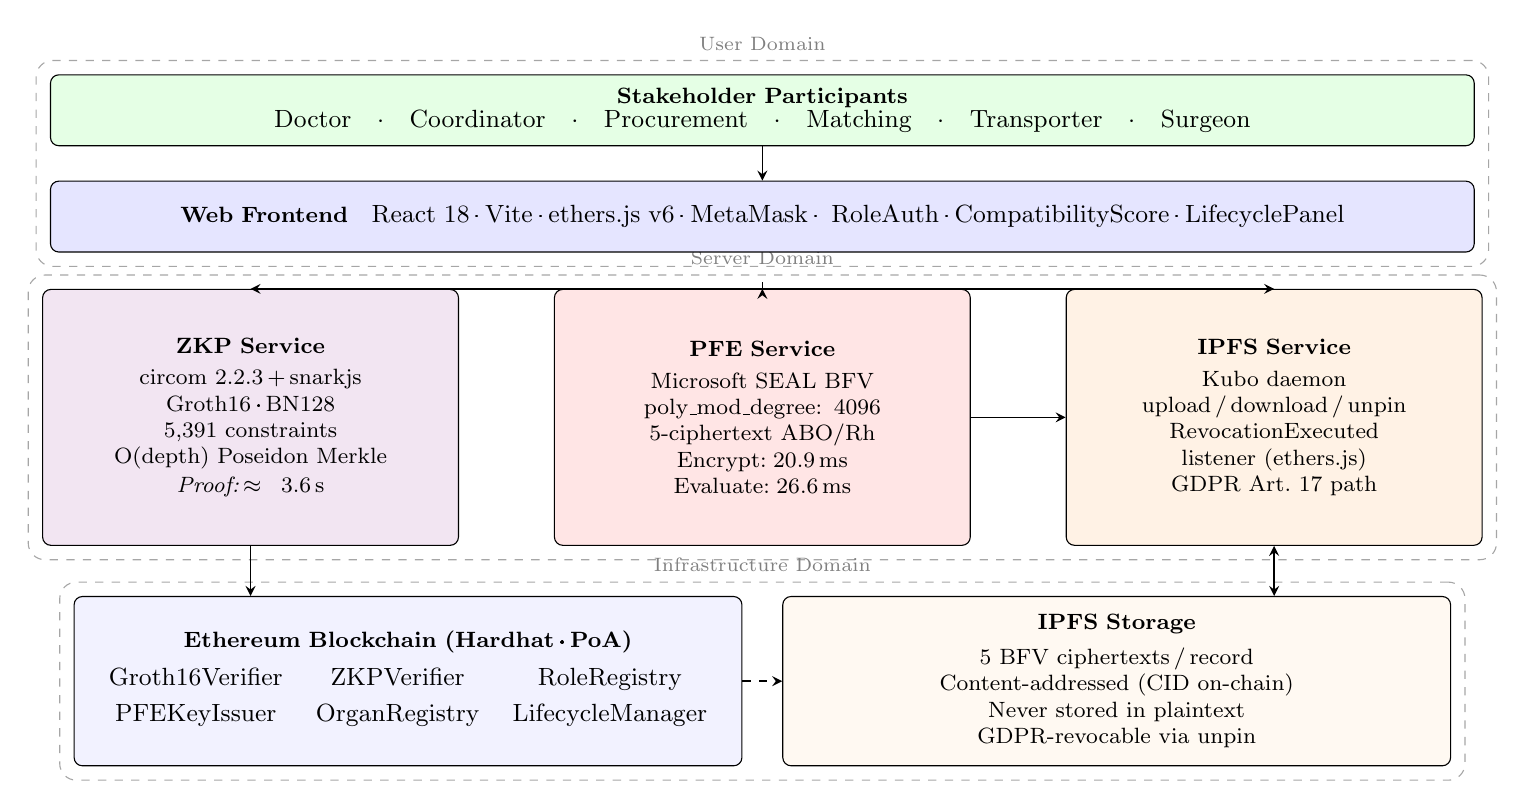
\begin{tikzpicture}[
  x=1cm,y=1cm,
  every node/.style={align=center,font=\footnotesize},
  wb/.style={draw,rounded corners=3pt,text width=17.8cm,
             minimum height=0.9cm,fill=#1,inner sep=4pt},
  sb/.style={draw,rounded corners=3pt,text width=5.0cm,
             minimum height=3.25cm,fill=#1,inner sep=4pt},
  ib/.style={draw,rounded corners=3pt,text width=8.2cm,
             minimum height=2.15cm,fill=#1,inner sep=4pt},
  arr/.style={->,>=stealth,semithick},
  darr/.style={->,>=stealth,semithick,dashed},
  dl/.style={draw,dashed,rounded corners=6pt,gray!70,inner sep=5pt}
]

% ---- Row 1: Participants ----
\node[wb=green!10] (PAR) at (9.5,8.9)
  {\textbf{Stakeholder Participants}\\[-1pt]
   \small Doctor\quad$\cdot$\quad Coordinator\quad$\cdot$\quad Procurement\quad$\cdot$\quad
   Matching\quad$\cdot$\quad Transporter\quad$\cdot$\quad Surgeon};

% ---- Row 2: Frontend ----
\node[wb=blue!10] (FE) at (9.5,7.55)
  {\textbf{Web Frontend}\quad
   \small React~18\,·\,Vite\,·\,ethers.js~v6\,·\,MetaMask\,·\,
   RoleAuth\,·\,CompatibilityScore\,·\,LifecyclePanel};

% ---- Row 3: Backend services ----
\node[sb=violet!10] (ZKP) at (3.0,5.0)
  {\textbf{ZKP Service}\\[2pt]
   circom~2.2.3\,+\,snarkjs\\
   Groth16\,·\,BN128\\
   5{,}391 constraints\\
   O(depth) Poseidon Merkle\\[1pt]
   \textit{Proof:}\;\!$\approx\!3.6$\,s};

\node[sb=red!10] (PFE) at (9.5,5.0)
  {\textbf{PFE Service}\\[2pt]
   Microsoft SEAL~BFV\\
   poly\_mod\_degree: 4096\\
   5-ciphertext ABO/Rh\\
   Encrypt:\;20.9\,ms\\
   Evaluate:\;26.6\,ms};

\node[sb=orange!10] (IPFSSVC) at (16.0,5.0)
  {\textbf{IPFS Service}\\[2pt]
   Kubo daemon\\
   upload\,/\,download\,/\,unpin\\
   RevocationExecuted\\
   listener (ethers.js)\\
   GDPR~Art.~17 path};

% ---- Row 4: Infrastructure ----
\node[ib=blue!5] (ETH) at (5.0,1.65)
  {\textbf{Ethereum Blockchain (Hardhat\,·\,PoA)}\\[3pt]
   \small
   \begin{tabular}{@{}ccc@{}}
     Groth16Verifier & ZKPVerifier & RoleRegistry\\[2pt]
     PFEKeyIssuer & OrganRegistry & LifecycleManager
   \end{tabular}};

\node[ib=orange!5] (IPFSSTO) at (14.0,1.65)
  {\textbf{IPFS Storage}\\[3pt]
   5 BFV ciphertexts\,/\,record\\
   Content-addressed (CID on-chain)\\
   Never stored in plaintext\\
   GDPR-revocable via unpin};

% ---- Arrows ----
\draw[arr] (PAR.south) -- (FE.north);

\draw[arr] (FE.south |- ZKP.north) -- (ZKP.north);
\draw[arr] (FE.south |- PFE.north) -- (PFE.north);
\draw[arr] (FE.south |- IPFSSVC.north) -- (IPFSSVC.north);

\draw[arr] (ZKP.south) -- (ZKP.south |- ETH.north);
\draw[arr] (PFE.east) -- (IPFSSVC.west);

\draw[arr,<->] (IPFSSVC.south) --
  (IPFSSVC.south |- IPFSSTO.north);

\draw[darr] (ETH.east) -- (IPFSSTO.west);

% ---- Domain boxes ----
\begin{pgfonlayer}{background}
  \node[dl,fit=(PAR)(FE),
    label={[gray,font=\scriptsize]above:User Domain}] {};
  \node[dl,fit=(ZKP)(PFE)(IPFSSVC),
    label={[gray,font=\scriptsize]above:Server Domain}] {};
  \node[dl,fit=(ETH)(IPFSSTO),
    label={[gray,font=\scriptsize]above:Infrastructure Domain}] {};
\end{pgfonlayer}

\end{tikzpicture}%
}
\caption{Three-tier architecture of the proposed system. Solid arrows denote data
flows; the dashed arrow denotes the GDPR Art.~17 revocation event
(\texttt{LifecycleManager} $\rightarrow$ IPFS unpin).}
\label{fig:arch}
\end{figure*}

%% ══════════════════════════════════════════════════════════════════════════════
\section{Preliminary Implementation}
\label{sec:impl}
%% ══════════════════════════════════════════════════════════════════════════════

\subsection{Technology Stack}

Table~\ref{tab:stack} summarises the prototype technology stack.

\begin{table}[!t]
\centering
\caption{Implementation technology stack.}
\label{tab:stack}
\renewcommand{\arraystretch}{1.15}
\scriptsize
\setlength{\tabcolsep}{4pt}
\begin{tabularx}{\columnwidth}{>{\raggedright\arraybackslash}p{2.0cm} X}
\toprule
\textbf{Component} & \textbf{Technology} \\
\midrule
Blockchain    & Hardhat~2.x, Solidity~0.8.20 (EVM Paris), PoA \\
ZKP circuit   & circom~2.2.3, snarkjs~0.7.4, Groth16/BN128 \\
Hash function & Poseidon (ZK-friendly, circomlibjs) \\
HE scheme     & Microsoft SEAL via node-seal (BFV) \\
IPFS storage  & Kubo daemon, ipfs-http-client \\
Frontend      & React~18, Vite, ethers.js~v6 \\
Backend API   & Express~4, Node.js~20 \\
Testing       & Hardhat test, chai, circom\_tester \\
\bottomrule
\end{tabularx}
\end{table}

\subsection{ZKP Circuit Design}

The \texttt{roleProof.circom} template instantiates three \texttt{Poseidon(2)} components
for nullifier, commitment, and leaf-hash computation, plus one \texttt{MerkleProof(20)}
component~(20 levels of \texttt{Mux1} selector + \texttt{Poseidon(2)} per level).
Total: 5,\!391 constraints. The circuit was compiled using circom~2.2.3
with the \texttt{r1cs}, \texttt{wasm}, and \texttt{sym} outputs.
A Powers-of-Tau ceremony~(\texttt{ptau~12}) and phase-2 specialisation produced
the \texttt{.zkey} proving key~(5.2\,MB).

A critical performance optimisation replaced the naïve O($2^\ell$) Merkle tree
build~(hashing all~$2^{20} \approx 10^6$ leaves pairwise, taking~$\approx\!60$\,s in
circomlibjs) with the standard \emph{cached-zero-subtree} technique~(used by Tornado
Cash and Semaphore): precompute the hash of an all-zero subtree at each level~(20
Poseidon calls), then walk only the credential's path~(20 more calls), reducing tree
build time from~60\,s to~$\approx\!5$\,ms with mathematically identical outputs.

\subsection{BFV Compatibility Polynomial Implementation}

The five-ciphertext ABO/Rh decomposition evaluates blood-type incompatibility as
three independent single-depth BFV multiplications (same multiplicative depth as the
original three-variable scheme), ensuring no change to BFV cryptographic parameters.
Verified with hand-computed reference values across all 64 blood-type pair
combinations and multiple HLA scenarios. Two representative results~(illustrative
values):

\begin{center}
\scriptsize
\begin{tabularx}{0.92\columnwidth}{>{\raggedright\arraybackslash}X c}
\toprule
\textbf{Scenario} & \textbf{Score} \\
\midrule
O$^-$ donor + O$^-$ recipient, HLA~85\% match & $\approx\!970$\,/\,1000 \\
B$^+$ donor + O$^-$ recipient, HLA~80\% match & $\approx\!650$\,/\,1000 \\
\bottomrule
\end{tabularx}
\end{center}

\noindent The B$^+\to$O$^-$ scenario correctly reflects ABO incompatibility (B donor
cannot donate to O recipient): previously it scored 1000/1000 due to single-bit
blood-type encoding in the baseline approach.

\subsection{Test Coverage and Benchmark Results}

The test suite comprises 62 fast unit and PFE-integration tests~(2\,s) and
10~integration tests requiring real Groth16 proof generation and IPFS access.
All 62/62 fast tests pass; 69--72/72 with integration tests~(IPFS tests skip
gracefully without a running daemon).

Table~\ref{tab:bench} reports measured performance on an Intel~i7-12700H,
16\,GB RAM, Windows~11, Node.js~22.

\begin{table}[!t]
\centering
\caption{Measured performance benchmarks (10-iteration means where applicable).}
\label{tab:bench}
\renewcommand{\arraystretch}{1.15}
\scriptsize
\setlength{\tabcolsep}{3pt}
\begin{tabularx}{\columnwidth}{>{\raggedright\arraybackslash}X >{\raggedleft\arraybackslash}p{1.45cm} >{\centering\arraybackslash}p{0.8cm}}
\toprule
\textbf{Metric} & \textbf{Value} & \textbf{Unit} \\
\midrule
Merkle tree build (naïve, O($2^{20}$)) & 59{,}680 & ms \\
Merkle tree build (cached zeros, O(depth)) & $\approx\!5$ & ms \\
Groth16 proof generation & 3{,}640.6 & ms \\
\texttt{verifyAndIssueKey} gas & 375{,}645 & gas \\
SEAL BFV encrypt (5 ciphertexts) & 20.9 & ms \\
SEAL BFV polynomial evaluate & 26.6 & ms \\
SEAL BFV decrypt & 1.5 & ms \\
\texttt{registerDonor} gas & 199{,}169 & gas \\
\texttt{executeRevocation} gas & 98{,}921 & gas \\
\bottomrule
\end{tabularx}
\end{table}

\textit{Merkle tree note:} The~60\,s naïve build is a pure-JavaScript circomlibjs
limitation~(not a proving-system bottleneck). The O(depth) fix reduces this to
$\approx\!5$\,ms. In production, credential registration is a one-time setup per
participant; per-authentication latency is dominated by proof generation~(3.6\,s).

\textit{Gas note:} At a 5\,Gwei base fee on a PoA network, 375,\!645\,gas $\approx$
0.00188\,ETH\,$\approx$\,\$5.64 at \$3{,}000/ETH~(Sepolia: effectively~\$0). On a
permissioned PoA chain, gas is configurable to near-zero cost.

\subsection{Prototype Trust Assumption}

In the current prototype, the credential~$c$ is transmitted to the Express backend over
HTTPS for server-side Merkle tree construction and proof generation. This is a stated
\emph{prototype engineering simplification}, not a cryptographic weakness: the proof's
zero-knowledge guarantee holds regardless of where proof generation executes. The
credential is not persisted and is discarded after proof generation. The production
hardening path~(client-side WASM proof generation using browser-compiled circom/snarkjs)
eliminates this trust assumption without modifying any contract or circuit.

%% ══════════════════════════════════════════════════════════════════════════════
\section{Security Analysis}
\label{sec:security}
%% ══════════════════════════════════════════════════════════════════════════════

\subsection{ZKP Soundness and Zero-Knowledge}

Groth16 under BN128 provides \emph{computational soundness} under the
$q$-Power Knowledge of Exponent assumption and \emph{computational zero-knowledge}
via the Groth16 simulator~\cite{groth16}. The honest verifier learns only: the
Groth16 proof is valid for the submitted public inputs. In particular, the credential,
salt, and Merkle path are never revealed.

\subsection{Replay Attack Prevention}

The nullifier~$\mathrm{Poseidon}(c, r)$ uniquely identifies each authentication
session. \texttt{PFEKeyIssuer} stores every used nullifier in the
\texttt{usedNullifiers} mapping; Check~3 rejects any proof reusing a prior nullifier.
The four-hour key TTL prevents indefinite key reuse. Both properties are verified by
integration test steps~9 and~10.

\subsection{GDPR Compliance Analysis}

\textbf{Art.~5(1)(f) (Integrity and confidentiality):} No plaintext attribute appears
on-chain or on IPFS; all records are BFV-encrypted. On-chain data consists only of
CID strings, permission bitmasks, and pseudonymous Ethereum addresses.

\textbf{Art.~5(1)(b) (Data minimisation):} Role-scoped PFE keys enforce data
minimisation at the cryptographic level: a Transporter key evaluates only
urgency/location terms, not donor identity or HLA data.

\textbf{Art.~17 (Right to Erasure):} \texttt{LifecycleManager.executeRevocation}
triggers IPFS unpinning. The CID and event log remain on-chain as the legally required
audit trail; only the data content is deleted.

\textbf{Art.~4(5) (Pseudonymisation):} ZKP role authentication decouples Ethereum
address from real-world identity. An adversary observing on-chain activity learns only
that a valid ZKP proof for roleId~$r$ was submitted at a given time; they cannot link
this to a specific credential or person.

%% ══════════════════════════════════════════════════════════════════════════════
\section{Conclusion and Future Work}
\label{sec:conclusion}
%% ══════════════════════════════════════════════════════════════════════════════

This Phase~II report presented a detailed architecture and working prototype for a
ZKP-authenticated, PFE-gated, IPFS-backed organ donation system on a permissioned
Ethereum blockchain. The system addresses five research gaps identified in Phase~I:
ZKP proof gating PFE key issuance~(Gap~1), antigen-level ABO/Rh homomorphic
compatibility~(Gap~2), GDPR Art.~17 lifecycle management~(Gap~3), end-to-end
IPFS-PFE organ pipeline~(Gap~4), and post-quantum cryptography~(Gap~5, planned).

Key measured results confirm feasibility: on-chain Groth16 verification costs
375,\!645 gas, BFV encryption runs in 20.9\,ms, and polynomial evaluation in 26.6\,ms.
The Merkle-tree O(depth) optimisation demonstrates practical protocol engineering:
a 12{,}000$\times$ reduction~(60\,s to 5\,ms) with mathematically identical
cryptographic output.

The primary open tasks are: (i)~Sepolia testnet deployment~(script and \texttt{.env}
prepared); (ii)~browser-side WASM proof generation~(eliminating the server-side trust
assumption); (iii)~extension of the compatibility polynomial to seven clinical
variables~(adding cold ischaemia time and geographic proximity);
(iv)~replacement of ECDSA with CRYSTALS-Dilithium~(ML-DSA-65, FIPS~204) for
post-quantum transaction authentication; and (v)~multi-hospital consortium deployment
at national-registry scale.

%% ── References ────────────────────────────────────────────────────────────────
\bibliographystyle{IEEEtran}
\bibliography{references}

\end{document}
